\section{PAGRINDINIAI MATŲ ATRINKIMO METODAI}

Dėl ,,daugiamatiškumo prakeiksmo`` (angl. \textit{the curse of dimentionality}) -- didėjant matų kiekiui mėginiai pasidaro panašūs, todėl bandymas juos klasifikuoti tolygus spėliojimui \cite{bellman1966adaptive}. Biomedicininių duomenų kontekste galima daryti prielaidą, kad ne visi matai yra susiję su tiriama problema, pvz. gaubtinės žarnos vėžiu, dėl to, kad duomenys yra daugiamačiai. Paprastai nagrinėjamai problemai svarbus yra mažas, palyginus su visu, matų kiekis. Todėl biomedicininių duomenų daugiamatiškumui sumažinti yra naudojami informatyviausių matų atrinkimo metodai \cite{guyon2003introduction} (angl. \textit{feature selection}). Matų atrinkimas yra svarbi biomedicininių duomenų apdorojimo (angl. \textit{preprocessing}) etapo dalis. Naudojant matų atrinkimo metodus, galima kovoti su daugiamatiškumo prakeiksmu matų skaičių priartinant prie mėginių skaičiaus. Todėl svarbu yra pasirinkti geriausiai tinkančią matų atrinkimo strategiją. Kadangi ir pačių matų atrinkimo metodų veikimas priklauso nuo konkrečių duomenų, tai metodo pasirinkimas yra sudėtinga užduotis.

Pagal tai, kaip matų atrinkimo metodai yra susiję su klasifikatoriumi, matų atrinkimo metodus galima skirstyti į tris kategorijas \cite{saeys2008robust}:
\begin{enumerate}
 \item Filtruojantys metodai (angl. \textit{filter methods}), pvz. \textit{Fisher} įvertis. Jie dirba tiesiogiai su duomenimis, o jų darbo rezultatas gali būti matų įvertinimas svoriais, matų reitingavimas ar tiesiog geriausių matų poaibis, kuriuo remiantis vėliau apmokomas klasifikatorius. Tokių metodų pagrindinis privalumas yra tai, kad jie yra greiti, tinka paskirstytų skaičiavimų aplinkoms ir nepriklausomi nuo klasifikavimo  metodo, tačiau remiantis atrinktaisiais matais nebūtinai bus sukurtas geriausias klasifikatorius.
 \item Prisitaikantieji metodai (angl. \textit{wrapper methods}). Pirma, apmokomas klasifikatorius su visais matais, antra, parenkamas matų poaibis ir apmokomas klasifikatorius. Po daugkartinio matų aibių įvertinimo pagal klasifikavimo rezultatus yra nusprendžiama, kuris matų poaibis yra labiausiai tinkamas klasifikavimui. Įterptinių metodų atveju matų atrinkimo procesas yra neatsiejamas nuo klasifikavimo proceso -- matai yra atrenkami pagal klasifikatoriaus darbo rezultatus. Prisitaikantieji metodai dažnai duoda geresnius rezultatus negu filtravimo metodai, bet yra reiklūs resursams.
 \item Įterptiniai metodai (angl. \textit{embedded methods}), pvz. AW-SVM\cite{vapnik2000nature}. Jie matų atrinkimui naudoja vidinius klasifikatoriaus duomenis (pvz. matų svoriai gauti pagal SVM). Šie metodai dažnai siūlo gerą santykį tarp klasifikavimo tikslumo ir skaičiavimų sudėtingumo.
\end{enumerate}

Šiame skyriuje nagrinėsiu pagrindinius matų atsirinkimo metodus:
\begin{enumerate}
 \item \textit{Fisher} įvertis (angl. \textit{Fisher ratio})\cite{Pavlidis:2001:GFC:369133.369228};
 \item \textit{Relief} metodas\cite{DBLP:journals/ml/Robnik-SikonjaK03};
 \item Asimetrinis priklausomybės koeficientas (angl. \textit{Asymmetric Dependency Coefficient, ADC}) \cite{Shannon:2001:MTC:584091.584093};
 \item Absoliučių svorių SVM (angl. \textit{Absolute Weight SVM}, AW-SVM) \cite{vapnik2000nature};
 \item Rekursyvus matų eliminavimas pagal SVM (SVM-RFE) (angl. \textit{Recursive Feature Elimination by SVM}) \cite{Guyon:2002:GSC:599613.599671}.
\end{enumerate}

\subsection{\textit{Fisher} įvertis}

\textit{Fisher} įvertis vertina individualius matus pagal matų klasių atskiriamąją galią. Mato įvertis yra sudarytas iš tarpklasinio skirtumo santykio su vidiniu klasės pasiskirstymu:
\begin{equation}
 FR(j) = \frac{(\mu_{j1} - \mu_{j2})^2}{\sigma_{j1}^2 + \sigma_{j2}^2},
\end{equation}
kur, 
$j$ -- yra mato indeksas, 
$\mu_{jc}$ -- mato $j$ reikšmių vidurkis klasėje $c$, 
$\sigma_{jc}^2$ -- mato $j$ reikšmių standartinis nuokrypis klasėje $c$, kur $c={1,2}$. Kuo didesnis yra \textit{Fisher} įvertis, tuo geriau ts matas atskiria klases. Nors ir paprastas, šis metodas neįvertina matų tarpusavio sąveikų.

\subsection{\textit{Relief} metodas}

\textit{Relief} metodas iteratyviai skaičiuoja matų ,,susietumą``. Pradžioje ,,susietumas`` visiems matams yra lygus nuliui. Kiekvienoje
iteracijoje atsitiktinai pasirenkamas mėginys iš mėginių aibės, surandami artimiausi kaimynai iš tos pačios ir kitos grupių, ir atnaujinamos visų 
matų ,,susietumo`` reikšmės. Dėl atsitiktinumo faktoriaus klasifikavimo ir  matų atrinkimo stabilumo rezultatai naudojant šį metodą varijuoja. Mato įvertis yra vidurkis visų objektų atstumų skirtumų iki artimiausių kaimynų iš kitos ir tos pačios klasių:
\begin{equation}
 W(j)=W(j) - \frac{diff(j, x, x_H)}{n} + \frac{diff(i, x, x_M)}{n},
\end{equation}
kur 
$W(j)$ -- $j$-ojo mato ,,susietumo`` įvertis, 
$n$ -- mėginių aibės dydis, 
$x$ -- atsitiktinai pasirinktas mėginys, 
$x_H$ - artimiausias $x$ kaimynas iš tos pačios grupės (angl. \textit{nearest-Hit}), 
$x_M$ -- artimiausias $x$ kaimynas iš kitos grupės (angl. \textit{nearest-Miss}),
$diff(j, x, x')$ -- $j$-ojo mato reikšmių skirtumas tarp atsitiktinai pasirinkto objekto $x$ ir atitinkamo jo kaimyno, kur skirtumą į intervalą $[0, 1]$ normalizuojanti funkcija yra:
\begin{equation}
 diff(j, x, x')=\frac{|x_j- x_j'|}{x_{j_{max}} - x_{i_{min}}},
\end{equation}
kur $x_{j_{max}}$ ir $x_{j_{min}}$ yra maksimali ir minimali $j$-ojo matų reikšmės. ,,Susietumo`` reikšmių atnaujinimas yra vykdomas $n$ kartų ir kuo didesnė galutinė reikšmė, tuo svarbesnis matas. Šis algoritmas atsižvelgia į matų tarpusavio priklausomybes, nes mėginio artimiausias kaimynas yra ieškomas pagal visus mėginį apibūdinančius matus. Aprašyta algoritmo versija yra skirta dviejų klasių atvejui, tačiau yra ir multiklasinis algoritmo variantas \cite{DBLP:journals/ml/Robnik-SikonjaK03}.

\subsection{Asimetrinis priklausomybės koeficientas}

Asimetrinis priklausomybės koeficientas (angl. \textit{asymetric dependency coefficient}, ADC) yra matų reitingavimo motodas, kuris matuoja mėginio grupės tikimybinę priklausomybę $j$-ajam matui, naudodamas informacijos prieaugį (angl. \textit{information gain}) \cite{kent1983information}:
\begin{equation}
 ADC(Y, j) = \frac{MI(Y, X_j)}{H(Y)},
\end{equation}
kur $H(Y)$ -- klasės $Y$ entropija (angl. \textit{entropy}), o $MI(Y, X_j)$ -- yra tarpusavio informacija \cite{Shannon:2001:MTC:584091.584093} (angl. \textit{mutual information}) tarp mėginio grupės $Y$ ir $j$-ojo mato.
\begin{equation}
 H(Y)=-\sum_y{p(Y=y)log{p(Y=y)}}, 
\end{equation}
\begin{equation}
 H(X_j)=-\sum_x{p(X_j=x) log{p(X_j=x)}},
\end{equation}
\begin{equation}
 MI(Y, X_j) = H(Y) + H(X_j) - H(Y, X_j),
\end{equation}
\begin{equation}
 H(Y, X_j) = -\sum_{y,x_j}{p(y, x_j)log{p(y, x_j)}},
\end{equation}
Kuo didesni ADC įverčiai, tuo matas yra svarbesnis, nes turi daugiau informacijos apie mėginio priklausomybę grupei.

\subsection{Absoliučių svorių SVM}

Atraminių vektorių klasifikatorius (SVM) yra vienas populiariausių klasifikavimo algortimų, nes jis gerai susidoroja su daugiamačiais duomenimis \cite{guyon2002gene}. Yra keletas bazinių SVM variantų \cite{vapnik2000nature}, bet šiame darbe naudosime tiesinį SVM, nes jis demonstruoja gerus rezultatus analizuojant genų ekspresijos duomenimis. Tiesinis SVM yra hiperplokštuma apibrėžta kaip:
\begin{equation}
 \sum_{j=1}^{p}{w_jx_j + b_0 = 0},
\end{equation}
kur $p$ -- matų kiekis, $w_j$ -- j-ojo mato svoris, $x_j$ -- j-ojo mato kintamasis, $b_0$ -- konstanta. Mato absoliutus svoris $w_j$ gali būti panaudotas
matų reitingavimui. Svorį reikia imti absoliutaus dydžio, nes neigiamas svoris implikuoja priklausomybę vienai grupei, o teigiamas kitai grupei. Pastebėtina, kad svorių nustatymas yra atliekamas tik vieną kartą (SVM-RFE matų atrinkimo metodas svorius matams nustato daug kartų).

\subsection{Rekursyvus matų eliminavimas pagal SVM}

Rekursyvus matų eliminavimas pagal SVM (angl. \textit{Support Vector Machines -- Recursive Feature Elimination}, SVM-RFE) yra vienas populiariausių matų atrinkimo algoritmų \cite{guyon2002gene}. Todėl, jis yra naudojamas kaip atskaitos taškas (angl. \textit{benchmark}) vertinant kitus matų atrankos metodus. Iš esmės šis metodas yra daugkartinis absoliučių svorių SVM metodo taikymas nuolat išmetinėjant matus su mažiausiais svoriais. Rekursyvus matų eliminavimas mums padeda surasti tinkamą matų poaibį, kas ne visada pavyksta su matų reitingavimo metodais. Bendroji rekursyvaus matų eliminavimo procedūra:
\begin{algorithm}
\caption{Rekursyvus matų eliminavimas}
\label{RFE}
 \begin{enumerate}
 \item Turime pilną matų rinkinį $F_0$, nustatome $i=0$;
 \item Įvertiname kiekvieno mato kokybę matų aibėje $F_i$;
 \item Išmetame mažiausiai kokybišką matą iš $F_I$ tam, kad gautume matų rinkinį $F_{i+1}$;
 \item Nustatome $i=i+1$ ir grįžtame į antrąjį žingsnį kol nėra patenkinta algoritmo pabaigos sąlyga.
\end{enumerate}
\end{algorithm}
Jei trečiajame algoritmo žingsnyje iš matų aibės yra pašalinamas tik viena matas, tai gauname matų reitingavimą, o jei pašalinamas fiksuotas skaičius ar dalis (pvz. 50\%) matų, tai matų reitingavimo negauname. Pastebėtina, kad rekursyvus matų eliminavimas labai padidina algoritmo sudėtingumą. Algoritmo pabaigos sąlyga gali būti koks nors konkretus matų skaičius arba tiesiog matų aibę mažiname tol, kol matų visai nebeliks.

\section{STABILIŲ MATŲ ATRINKIMO METODAI}
\label{stabiliu_matu_atrinkimo_metodai}

Naudodami matų atrinkimo metodus, biomedicininius duomenis tiriantys mokslininkai susiduria su atrinktųjų matų aibės stabilumo problema - atrenkant matus pagal kitą mėginių poaibį, gaunamas kitas informatyviausių matų poaibis. Matų atrinkimo nestabilumas yra sąlygotas šių veiksnių:
\begin{enumerate}
 \item Duomenys yra triukšmingi ir kai kurie matai gali būti palaikyti informatyviais dėl atsitiktinių priežasčių;
 \item Daugiamačiuose duomenyse tikėtina, kad dalis matų koreliuoja, todėl, kuris iš koreliuojančių matų bus pasirinktas, priklauso nuo to, kuriuos mėginius pasirinksime klasifikatoriaus apmokymui;
 \item Kiekvienas maatų atrinkimo algoritmas daro skirtingas prielaidas apie tai, kurie matai yra informatyvūs.
\end{enumerate}
Galime teigti, kad skirtingi metodai tiems patiems duomenims gali atrinkti skirtingus matus. Taip pat, suskaidžius turimus duomenis į atskiras persidengiančias aibes ir atrinkus tą patį kiekį matų tuo pačiu metodu, gaunamos skirtingos matų aibės. Be to, kuo triukšmingesni duomenys, kuo mažiau turima mėginių ir kuo daugiau yra matų, tuo ryškesnė yra ši problema \cite{loscalzo2009consensus}. 

Vienas iš būdų didinti matų atrinkimo stabilumą yra naudoti multikriterinius matų atrinkimo metodus. Jų esmė yra panaudoti kelis matų atrinkimo metodus suliejant jų rezultatus į vieną bendrą rezultatą. Yra skiriamos trys priežastys, kodėl keletas agreguotų silpnų ir nestabilių matų atrinkimo metodų gali duoti stabilesnius matų atrinkimo rezultatus \cite{dietterich2000ensemble}:
\begin{enumerate}
 \item Keletas skirtingų, bet vienodai optimalių hipotezių gali būti teisingos, ir kriterijų agregavimas sumažiną tikimybę, kad bus pasirinkta neteisinga  hipotezė;
 \item Atskiri matų atrinkimo metodai gali dirbti skirtinguose lokaliuose optimumuose, tuo tarpu agregavimas gali geriau reprezentuoti tikrąją  duomenis generuojančią funkciją;
 \item Tikroji duomenų funkcija negali būti reprezentuojama jokia hipoteze paskiro algoritmo hipotezių erdvėje ir agreguojant pavienių metodų rezultatus galima praplėsti hipotezių erdvę.
\end{enumerate}
Apibendrinant galima sakyti, kad suliejant keletą skirtingų matų atrinkimo metodų rezultatų suliejamos gerosios pavienių matų atrinkimo metodų savybės, taip bandant kompensuoti tų algoritmų silpnybes.

Šiame skyriuje aptarsiu matų atrinkimo stabilumą didinančius metodus:
\begin{enumerate}
 \item Svoriais grįstas multikriterinis suliejimas;
 \item Reitingais grįstas multikriterinis suliejimas;
 \item Svoriais ir reitingais grįstas multikriterinis suliejimas;
 \item Multikriterinis rekursyvus matų eliminavimas;
 \item Konsensuso grupėmis grįstas stabilių matų atrinkimo metodas.
\end{enumerate}

\subsection{Svoriais grįstas multikriterinis suliejimas}

Svoriais grįsto multikriterinio matų atrinkimo suliejimo pagal svorius algoritmo pirmajame žingsnyje kiekvienas bazinis metodas priskiria duomenų rinkinio matams svorius, tada tie svoriai yra kombinuojami į vieną sutarties (angl. \textit{consensus}) svorių vektorių, kurio pagrindu yra gaunami matų reitingai. Algoritmas yra pavaizduotas ~\ref{fig:figure4} pav.
\begin{figure}
 \centering
 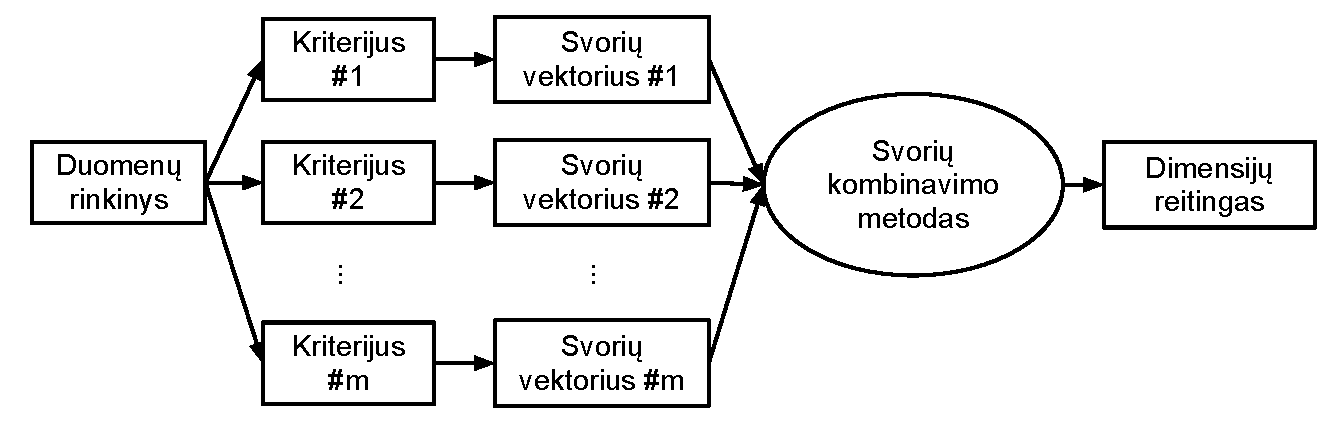
\includegraphics[width=1\textwidth]{images/score_based_fusion.pdf}
 \caption{Svoriais grįstas multikriterinis suliejimas.}
 \label{fig:figure4}
\end{figure}
\begin{figure}[ht]
\begin{minipage}[b]{0.5\linewidth}
\centering
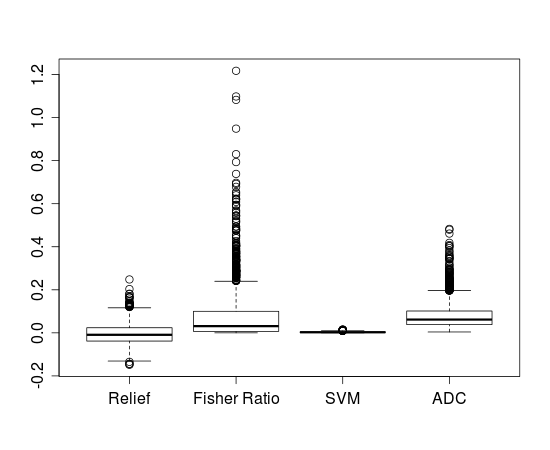
\includegraphics[width=1\textwidth]{images/boxplot_colon_all.png}
\caption{Pavienių matų atrinkimo metodų nenormalizuotas svorių pasiskirstymas.}
\label{fig:figure1}
\end{minipage}
\hspace{0.5cm}
\begin{minipage}[b]{0.5\linewidth}
\centering
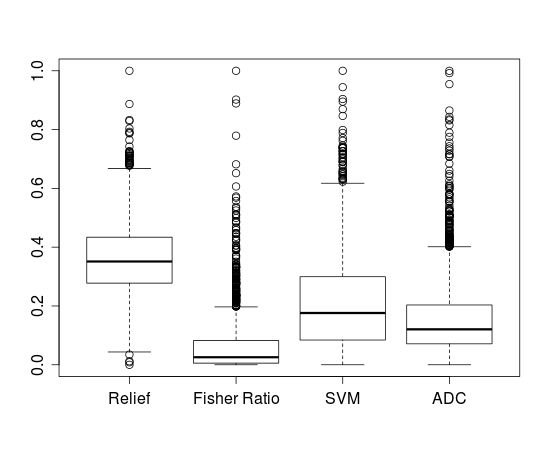
\includegraphics[width=1\textwidth]{images/boxplot_colon_all_normalized.png}
\caption{Pavienių matų atrinkimo metodų normalizuotas svorių pasiskirstymas.}
\label{fig:figure2}
\end{minipage}
\end{figure}

Suliejant svorius svarbu yra užtikrinti, kad svoriai, gauti naudojant skirtingus bazinius kriterijus, būtų palyginami. Todėl svorių normalizavimas turi būti atliekamas prieš svorių kombinavimą. Kitu atveju matų įvertinimai bus nepalyginami. Paveikslėlyje ~\ref{fig:figure1} pav. nenormalizuotų pavienių matų vertinimo metodų skiriasi netgi suteiktų svorių intervalai. Paveikslėlyje ~\ref{fig:figure2} pav. matome, kad net ir normalizavus svorius skiriasi svorių kvartiliai -- į tai reikia atkreipti dėmesį interpretuojant galutinius matų vertinimo rezultatus. Šiame darbe svoriai yra normalizuoti intervale $[0, 1]$ pagal formulę:
\begin{equation}
 u_i'=\frac{u_i - u_{i_{min}}}{u_{i_{max}} - u_{i_{min}}}, 
\end{equation}
kur $u_i$ - matų svorių vektorius pagal $i$ kriterijų, 
$u_{i_{min}}$ - minimali $u_i$ svorių vektoriaus reikšmė,
$u_{i_{max}}$ - maksimali $u_i$ svorių vektoriaus reikšmė,
$u_i'$ - normalizuotų svorių vektorius.

Sutarties svorių vektorius $u$ yra vidurkis normalizuotų svorių vektorių:
\begin{equation}
 u = \frac{1}{m}\sum_{i=1}^m u_i',
\end{equation}
kur $m$ yra bazinių kriterijų skaičius. Reikia paminėti, kad didesnė svorio reikšmė reiškia, kad matas yra reikšmingesnis klasifikavimui.

\subsection{Reitingais grįstas multikriterinis suliejimas}

Reitingais grįsto multikriterinio suliejimo pagal reitingus metodas gauna mėginių aibę aprašančių matų reitingą, pagal keletą bazinių matų reitingavimo kriterijų. Algoritmo pirmajame žingsnyje keletas matų atrinkimo kriterijų grąžina matų reitingus, paskui tie reitingai yra kombinuojami į vieną bendra matų reitingą. Algoritmas yra
pavaizduotas ~\ref{fig:figure5} pav.
\begin{figure}
 \centering
 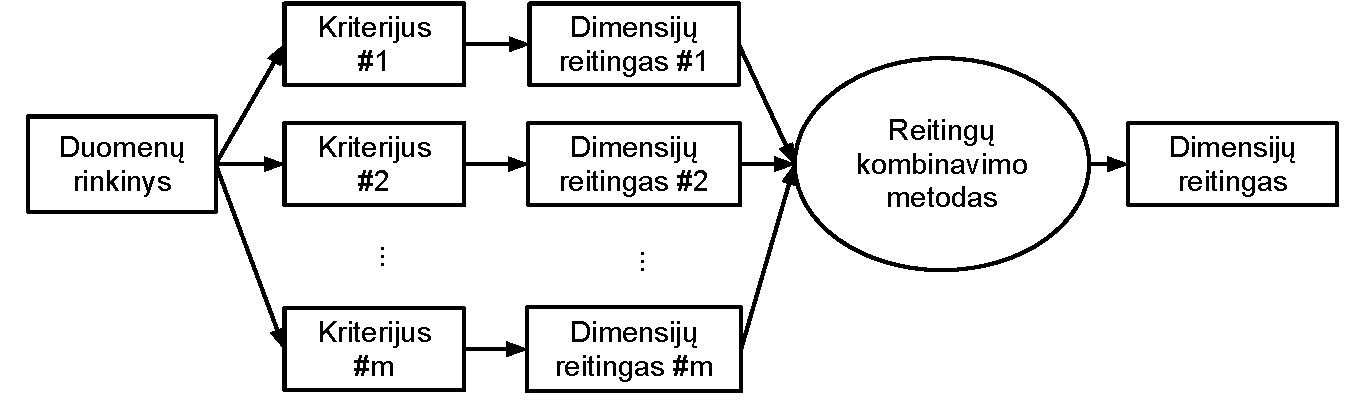
\includegraphics[width=1\textwidth]{images/ranking_based_fusion.pdf}
 \caption{Reitingais grįstas multikriterinis suliejimas.}
 \label{fig:figure5}
\end{figure}
Suliejimo pagal reitingus metodas nereikalauja matų atrinkimo metodų rezultatų normalizavimo, todėl galima matams priskirtus reitingus kombinuoti iškart. Skirtingai nei suliejimo pagal svorius algoritme, baziniai matų atrinkimo kriterijai turi gražinti matų reitingus, o ne svorius.

Matų reitingų kombinavimui yra keletas metodų\cite{dwork2001rank}, tačiau paprastumo dėlei šiame darbe naudosiu Borda balsavimą\footnote{Dar žinomas kaip ,,Pažymių metodas``. Jis buvo pasiūlytas prancūzų matematiko ir fiziko Jean-Charles de Borda 1770 metais.} (angl.\textit{ Borda count}). Tarkime, kad turime $m$ basuotojų ir $p$ kandidatų aibę. Tada Borda balsavimo metodas kiekvienam $i$-ajam balsuotojui sukuria balsų vektorių $v_i$ tokiu būdu: geriausiai įvertintam kandidatui suteikiama $p$ taškų, antrajam kandidatui $p-1$, ir t.t. Galutiniai taškai yra gaunami sudedant visų balsuotojų taškus
\begin{equation}
 v = \sum_{i=1}^m v_i,
\end{equation}
kur $v$ yra suminių taškų vektorius, o iš jo galime gauti ir galutinius matų reitingus.

\subsection{Svoriais ir reitingais grįstas multikriterinis suliejimas}

Svoriais ir reitingais grįsto multikriterinio suliejimo metodas nuo reitingais grįsto multikriterinio suliejimo metodo skiriasi tuo, kad kaip dar vienas matų reitingas yra panaudojamas svoriais grįsto multikriterinio matų atrinkimo metu gautas reitingas. Multikriterinio matų įverčių ir pagal svorius, ir pagal reitingus metodas vyksta trimis žingsniais:
\begin{enumerate}
  \item Gauname matų reitingus pagal $m$ pavienių matų atrinkimo motodų;
  \item Suliejame matų įverčius pagal svorius, taip gauname vieną matų reitingą;
  \item Reitinguojame matus pagal visus turimus $m+1$ pavienius reitingus.
\end{enumerate} 
Algoritmas yra pavaizduotas ~\ref{fig:figure3} pav.
\begin{figure}
 \centering
 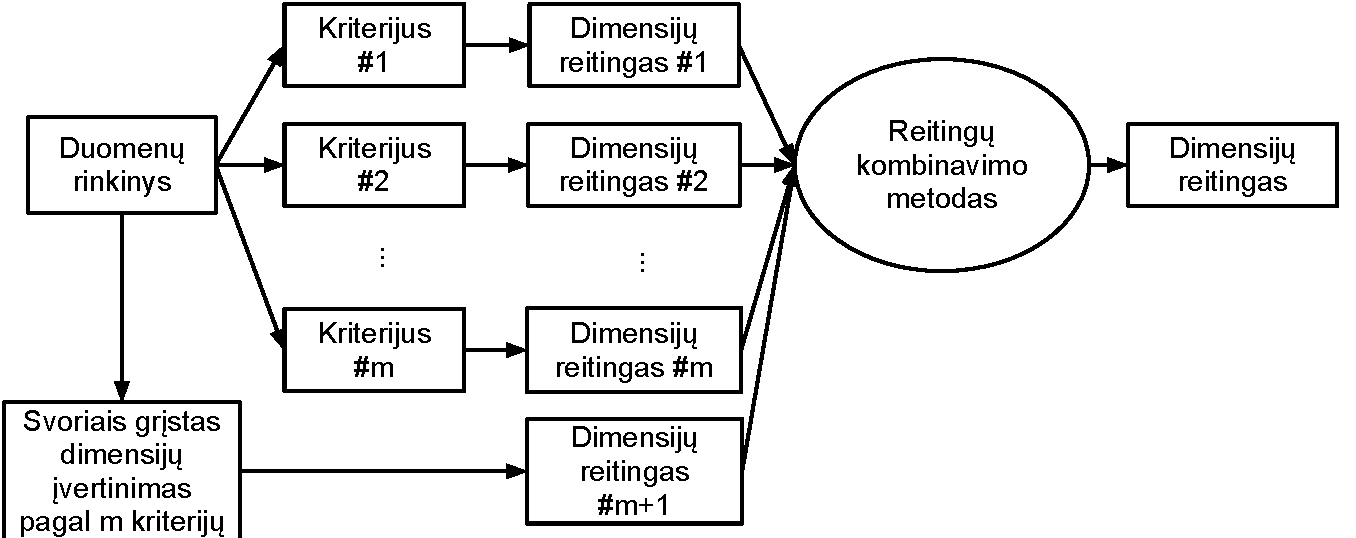
\includegraphics[width=1\textwidth]{images/score_and_ranking_based_fusion.pdf}
 \caption{Svoriais ir reitingais grįstas multikriterinis suliejimas.}
 \label{fig:figure3}
\end{figure}

Suliejami keletą mažai koreliuojančių matų reitingavimo metodų rezultatų, yra siekiama didesnio matų atrinkimo stabilumo, kai varijuoja treniravimosi duomenų poaibis (angl. \textit{subsampling}) \cite{yang2011robust}.

\subsection{Multikriterinis rekursyvus matų eliminavimas}

Jei matų atrinkimo tikslas yra pagerinti klasifikavimo rezultatus, tai taikymas multikriterinių matų atrinkimo metodų nebūtinai duos pageidaujamą rezultatą, nes yra pastebėta, kad vien matų reitingavimas nebūtinai suranda geriausią matų poaibį. Tam, kad būtų surastas geriausias matų poaibis reikia kombinuoti multikriterinį matų reitingavimą su matų paieškos strategija. Rekursyvus matų eliminavimas yra dažnai naudojama matų paieškos strategija matų atrinkimui. Todėl yra kombinuojamas multikriterinis matų reitingavimas ir rekursyvus matų eliminavimas.

Multikriterinis rekursyvus matų eliminavimas susideda iš dviejų dalių \cite{yang2011robust}: keletos matų atrinkimo kriterijų suliejimo pagal svorius ir pagal reitingus, ir rekursyvaus matų eliminavimo aprašyto algoritme nr. \ref{RFE}. Algoritmas pavaizduotas ~\ref{fig:figure6} pav.
\begin{figure}
 \centering
 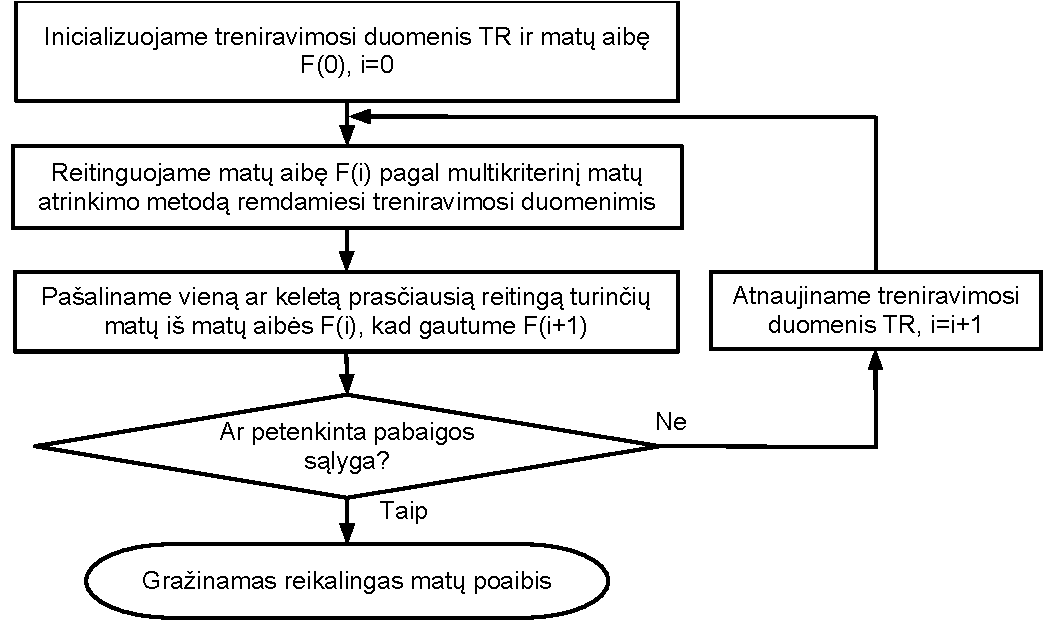
\includegraphics[width=0.7\textwidth]{images/mcf-rfe_procedure.pdf}
 \caption{Multikriterinio rekursyvaus matų eliminavimo algoritmas.}
 \label{fig:figure6}
\end{figure}

Standartinis rekursyvus matų eliminavimas, kai vienos iteracijos metu yra eliminuojamas vienas matas, gali labai padidinti algoritmo sudėtingumą. Todėl genų ekspresijos duomenims prasmingiau yra eliminuoti keletą matų vienu metu.

Nors SVM-RFE matų atrinkimo algoritmas ir yra labai populiarus, tačiau yra žinoma, kad jam trūksta stabilumo \cite{guyon2002gene}. Todėl kombinuodami didesnį stabilumą turintį multikriterinį matų atrinkimą su rekursyvaus matų eliminavimo paieškos strategija, gauname stabilesnį matų atrinkimo algoritmą.

\subsection{Konsensuso grupėmis grįstas stabilių matų atrinkimo metodas}

Konsensuso grupėmis grįstas stabilių matų atrinkimo metodas(angl. \textit{Consensus Group Stable feature selection}, CGS), pirma, identifikuoja panašių matų grupes, antra, pagal surastas grupes transformuoja matų aibę, trečia, transformuotoje matų aibėje atlieka matų atrinkimą \cite{loscalzo2009consensus}. Schematiškai šis algoritmas pavaizduotas ~\ref{fig:figure7} pav. 
\begin{figure}
 \centering
 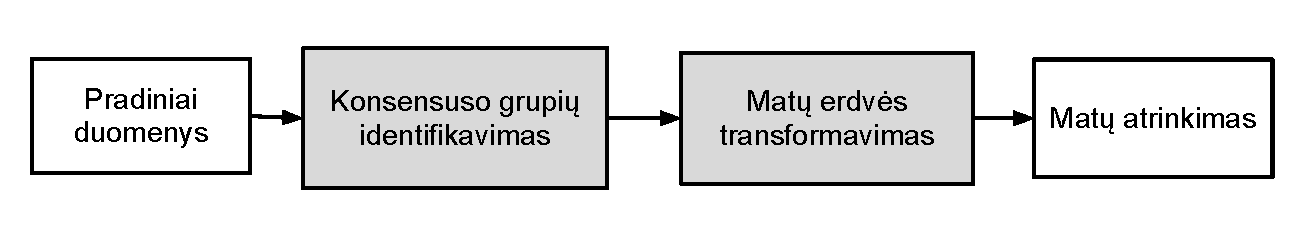
\includegraphics[width=\textwidth]{../bachelor/images/consensus_group_based_feature_selection_framework.pdf}
 \caption{Konsensuso grupėmis grįstas stabilių matų atrinkimas.}
 \label{fig:figure7}
\end{figure}

CGS metodo pagrindinė dalis yra panašių matų identifikavimas. Šio uždavinio sprendimui naudojamas \textit{Dense Group Finder} (DGF) algoritmas. DGF aprašytas algoritme nr. \ref{DGF}. CGS algoritme agal matai pagal DGF algoritmą yra sugrupuojami keletą kartų. Po pakartotinio grupavimo yra ieškoma stabilių grupių -- jei matas buvo sugrupuotas į konkrečią grupę daugiau nei pusėje grupavimų, tai matas ir priklausys tai konsensuso grupei. Matų aibės transformavimas vyksta iš kiekvienos konsensuso grupės išrenkant reprezentatyviausią matą -- konkretų matą esantį arčiausiai konsensuso grupės vidurkio. Išrinktieji reprezentatyviausieji matai ir sudaro transformuotą matų aibę. Transformuotoje matų aibėje vykdomas matų antrinkimas koriuo nors matų atrinkimo metodu $\Phi$, pavyzdžiui, \textit{Relief} matų atrinkimo metodu. 
\begin{algorithm}
\caption{DGF -- \textit{Dense Group Finder}}
\label{DGF}
 \begin{algorithmic}
 \item \textbf{Įeitis:} duomenys $D=\{x_i\}_{i=1}^n$, branduolio plotis $h$
 \item \textbf{Išeitis:} tankios matų grupės $G_1, G_1,..., G_L$
 \For{$i = 1$ \textbf{to} $n$ \do} 
  \State Inicializuojame $j=1, y_{i,j}=x_i$
  \Repeat
    \State Suskaičiuoti tankio centrą $y_{i, j+1}$ pagal (\ref{for_dgf})
  \Until{konverguoja}
  \State Nustatyti tankio centrą $y_{i,c} = y_{i,j+1}$ (Nustatyti piką $p_i$ kaip $y_{i,c}$)
  \State Sulieti piką $p_i$ su artimiausiais pikais, jei atstumai tarp jų $ < h$
 \EndFor
 \item Iš kiekvieno unikalaus piko $p_r$, pridėkime $x_i$ į $G_r$, jei $||p_r - x_i|| < h$
 \end{algorithmic}
\end{algorithm}

\begin{equation}
\label{for_dgf}
  y_{i, j+1}=\frac{\sum_{i=1}^{n} x_i K(\frac{y_j - x_i}{h})}{\sum_{i=1}^{n} K(\frac{y_j - x_i}{h})} j=1,2,...
\end{equation}
kur $K(x)$ -- \textit{kernel} funkcija, $h$ -- \textit{kernel} plotis, $y$ -- tankio centras.

\begin{algorithm}
 \caption{Konsensuso grupėmis grįstas stabilių matų atrinkimas}
 \label{CGS}
 \begin{algorithmic}
   \item \textbf{Įeitis:} mėginių aibė $D$, iteracijų skaičius $t$, matų atrinkimo metodas $\Phi$\
   \item \textbf{Išeitis:} atrinktos konsensuso matų grupės $CG_1, CG_1,..., CG_k$
   \item // Konsensuso grupių identifikavimas
   \For{$i = 1$ \textbf{to} $n$ \do}
    \State Parinkti mėginių  poaibį $D_i$ iš $D$
    \State Gauti panašių matų grupes pagal $DGF(D_i, h)$
   \EndFor
   \For{kiekvienai matų porai $X_i$ ir $X_j \in D$}
    \State Nustatyti $W_{i,j}=$ dažnis, kai $X_i$ ir $X_j$ yra toje pačioje grupėje $/t$
   \EndFor
   \item Sudaryti konsensuso grupes $CG_1, CG_1,..., CG_L$ atliekant hierarchinį klasterizavimą visiems matams pagal $W_{i, j}$
   \item //Matų atrinkimas grįstas konsensuso grupėmis
   \For{$i = 1$ \textbf{to} $l$ \do}
    \State Parinkti reprezentatyvų matą $X_i$ iš $CG_i$
    \State Įvertinti mato informatyvumą $\Phi(X_i)$
   \EndFor
   \item Reitinguoti konsensuso grupes $CG_1, CG_1,..., CG_L$ pagal $\Phi(X_i)$
   \item Pasirinkti $k$ matų, turinčių geriausią reitingą  
 \end{algorithmic}
\end{algorithm}